
In order to allow different scheduling strategies, we introduce the concept of
\emph{node priority} by assigning a priority value to every node in the program
and by introducing coordination facts that manipulate such priority values.  By
default, nodes have no priority and can be picked in any order. In our
implementation, we use a FIFO approach because older nodes tend to have a higher
number of unexamined facts, from which to derive subsequent new facts.

We have two kinds of priorities: a \emph{temporary priority} and a \emph{default
   priority}. A temporary priority momentarily changes the default priority $D$
of a node, so that once the node is done, the priority will default back to $D$.
Initially, all nodes have a default priority of $-\infty$.

The following list presents the action facts available to manipulate the
scheduling decisions of the system:

\begin{itemize}

   \item \code{set-priority(node A, float F)}: Sets the temporary priority of
      node \code{A} to \code{F}.  The programmer can decide if priorities
      are to be ordered in ascending or descending order, thus if node \code{A}
      has priority \code{G}, we only change it to \code{F} is \code{F > G}
      (ascending order) or \code{F < G} (descending order).

   \item \code{add-priority(node A, float F)}: Increases the temporary priority
      of node \code{A} by \code{F}.

   \item \code{remove-priority(node A)}: Removes the temporary priority from node
   \code{A}.

   \item \code{schedule-next(node A)}: Changes the temporary priority of node
   \code{A} to be $+\infty$.

   \item \code{set-default-priority(node A, float F)}: Sets the default
      priority of node \code{A} to \code{F}.

   \item \code{stop-program()}: Immediately stops the execution of the whole program.

\end{itemize}

LM also provides two sensing facts \code{priority(node A, float P)} and
\code{default-priority(node A, float P)}, which consult, respectively, the
temporary priority or default priority \code{P} of node \code{A}.  Sensing facts
can only be used in the body of rules and are exempt from the constraint that
forces every fact used in the body to have the same first argument. Also note
that when sensing facts are used to prove new facts, they are re-derived
automatically. All coordination facts are linear and thus consumed when used in
the body of a rule.  The system creates the necessary code to re-derive them
without programmer interaction. Likewise, \code{set-priority} and
\code{set-default-priority} update the value of \code{priority} facts by
retracting and re-asserting them but this is done implicitely by the runtime
system.

The priorities assigned to nodes are followed on a per-thread basis, therefore a
thread will always pick the highest priority node on its sub-graph but not the
highest priority node of the whole graph.
Figure~\ref{fig:coordination:priorities} shows an example of a graph being
processed by two threads, \code{T0} and \code{T1}. The order for \code{T0} will
be \code{@0}, \code{@1}, \code{@3}, \code{@2} and for thread \code{T1} it will
be \code{@4}, \code{@6}, \code{@5}. Priorities can also be seen as hints because
they do not provide a global ordering but only a per-thread ordering.

Note that priorities of nodes can be set from any node in the graph, even if those nodes
live on different threads. Of course, this implies communication between
threads.

\begin{figure}
\begin{center}
   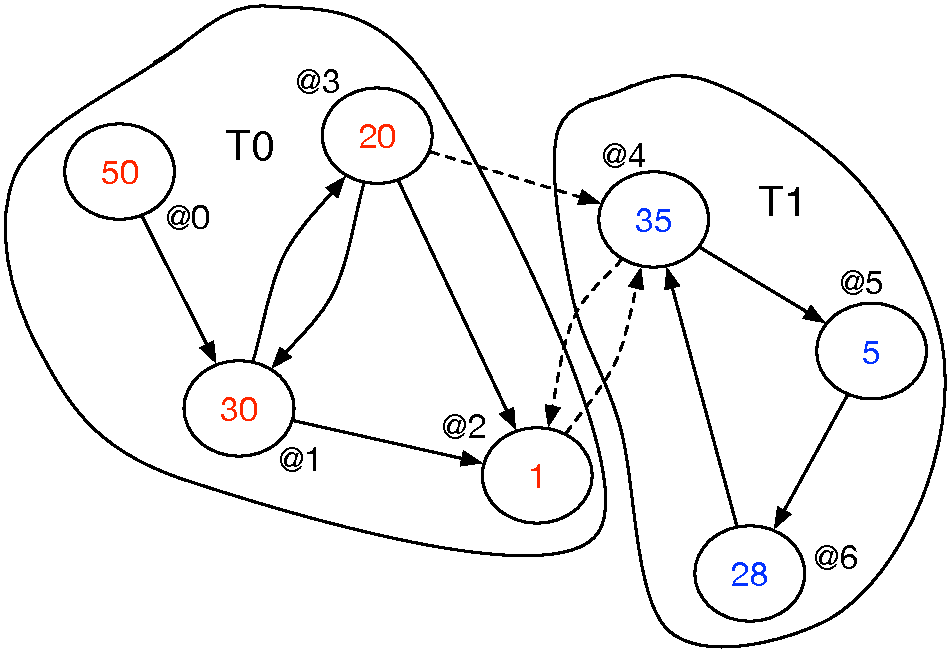
\includegraphics[width=0.6\textwidth]{figures/coordination/priorities.pdf}
\end{center}
\caption{Priorities with sub-graph partitioning. Priorities are used on a
   per-thread basis therefore thread \code{T0} schedules \code{@0} to
   execute, while \code{T1} schedules node \code{@4}.}
\label{fig:coordination:priorities}
\end{figure}
